% =====================================================================
%  Plan4ARI - Deliverable D4.1 (A4 revision)
%  Updated Scientific Plan for Local and Global Autonomous Motion Planning
%
%  Class: ../../../latex-style/plan4ari_report.cls (layout of the Plan4ARI D1.1 template)
%  Build: latexmk main.tex        (XeLaTeX, see latexmkrc)
%  Bibliography and MPPI SOTA body are shared with ../SOTA (LLM-wiki knowledge base)
% =====================================================================
\documentclass{plan4ari_report}

\usepackage{amsmath,amssymb,bm}
\usepackage{algorithm}
\usepackage{algpseudocode}
\usepackage{tikz}
\usetikzlibrary{arrows.meta,positioning,fit,backgrounds,calc}
\usepackage{cite}
\input{sota_macros}
\sotafullfalse%

\deliverable{D4.1}
\deliverabletitle{Scientific Plan and First Mockup of the Motion Planning Modules}
\docstatusline{Draft~-~Version 0.7}
\inforow{Project acronym}{Plan4ARI}
\inforow{Project duration}{48 months}
\inforow{Work package/activity}{Activity 4~-~Local and Global Autonomous Motion Planning}
\inforow{Task basis}{Task 4.1 Update of the Scientific Plan with the latest State-of-the-Art Methodologies and Tools for Motion Planning; Task 4.7 Benchmarking and Evaluation}
\inforow{Activity period}{M1--M6}
\inforow{Contractual delivery point}{M12}
\inforow{Document status}{Draft for internal review~-~Version 0.7}
\inforow{Lead beneficiary}{CNR}
\inforow{Dissemination level}{To be confirmed}

\begin{document}
\makecover%

\begin{documentcontrol}
\docversion{0.1}{20 July 2026}{TBC}{Initial draft outline}
\docversion{0.2}{1 June 2026}{N. Pedrocchi (CNR)}{State of the art (MPPI, path-wise redundancy, base placement)}
\docversion{0.4}{1 July 2026}{N. Pedrocchi (CNR)}{Revised architecture, benchmark plan}
\docversion{0.5}{1 October 2026}{N. Pedrocchi (CNR)}{MPPI evolution, path-wise redundancy, base placement, benchmark plan}
\docversion{0.6}{2 October 2026}{N. Pedrocchi (CNR)}{Structure aligned with D2.1; M12 delivery and mockup scope clarified}
\docversion{0.7}{2 October 2026}{N. Pedrocchi (CNR)}{Simulation environment design, repository reference and implementation milestones}
\docversion{1.0}{TBC}{TBC}{Approved deliverable}
\end{documentcontrol}

\subsection*{Approval record}
Approval is pending consortium review. The proposed methods and integration decisions in this draft do not constitute an approval record.

\subsection*{Purpose and boundary of this deliverable}
D4.1 comprises the updated scientific plan and the first mockup of the motion planning modules for Activity~4, due at M12 in the project deliverable schedule. Tasks~4.1 and~4.7 cover the scientific update and initial benchmark definition at M1--M6; this task period is distinct from the M12 delivery of D4.1. The mockup scope and evidence required for review are specified in Section~\ref{sec:mockup}. This draft does not establish that its demonstration or hardware validation has been completed. Tasks~4.2--4.6 will develop and integrate the modules; the contractual objectives and KPIs remain unchanged unless formally amended.

\sectionsonsamepage%
\tableofcontents%
\sectionsonnewpage%

\section{Executive summary}\label{sec:exec}

\begin{planbox}
D4.1 updates the scientific plan of Activity~4 with the state of the art that emerged after the submission of \PlanARI. The original pillars --- informed sampling-based planning with multi-path reuse (T4.2) and MPC micro-interpolation in the Core IPC (T4.3) --- are \textbf{retained}; an \textbf{MPPI-based look-ahead layer is added} between them, and the end-to-end pipeline is made explicit, starting from the \textbf{optimal localisation of the robot with respect to the task}.
\end{planbox}

Since the proposal, sampling-based motion planning has become fast enough to answer collision-free queries in microseconds on a standard CPU~\cite{thomason2024vamp}, and Model Predictive Path Integral (MPPI) control has matured into a practical, derivative-free receding-horizon method for manipulators and mobile robots, with open implementations and industrial adoption in the ROS\,2 navigation stack~\cite{williams2018tro,bhardwaj2021storm,macenski2023nav2survey}. A review of 119 sources (Sections~\ref{sec:method}--\ref{sec:software}) supports the following proposed decisions:
\begin{itemize}
\item \textbf{Sampling-based planning and MPPI.} MPPI is adopted as a \emph{stochastic look-ahead} that explores the task redundancy (tool roll, orientation tolerance, external axes, base) ahead of the robot, handles discrete configuration alternatives as multiple goals and reacts to scene changes. Sampling-based planning remains in charge of transfer motions, station-level feasibility and multi-path reuse (Section~\ref{sec:arch}).
\item \textbf{Explicit pipeline.} Scene model $\rightarrow$ task segmentation $\rightarrow$ optimal task localisation (stations, base, rail) $\rightarrow$ segment feasibility and cost-to-go $\rightarrow$ online execution (MPPI + transfers) $\rightarrow$ Core-IPC path--velocity MPC.
\item \textbf{Open IPC / Core IPC.} All stochastic computation runs in the Open IPC; the Core IPC receives smooth references and enforces hard limits and safety rules deterministically at 1\,kHz.
\item \textbf{Robot-agnostic framework.} Kinematic and task descriptions are inputs; inverse-kinematics solution classes generalise the classical eight solutions of spherical-wrist arms to cuspidal arms, extended joint ranges, external axes and mobile bases.
\item \textbf{Benchmarking (T4.7).} A catalogue of 17 applications; arc welding of large structures (reference demonstrator) is planned for validation on real hardware, \textbf{all other applications are planned for benchmarking in simulation}.
\end{itemize}
The expected effects are a reduction of reconfigurations and safety-induced idle time, constant process speed within tolerance, and portability across robot kinematics, while keeping the computation-time KPI comparable with the OMPL baseline of the proposal (CPU-first design).

\section{Objectives, scope and original baseline}\label{sec:objectives}

\subsection{Objectives of Activity 4}
Activity~4 develops motion planners for teams of mobile manipulators and industrial arms working in dynamic, human-shared environments, integrated in the COMAU MI.RA/Dexter platform and in the Core IPC. The project targets are autonomous plan generation in all working conditions (joint and Cartesian), a reduction of about 30\% of the execution time of interaction tasks with respect to state-of-the-art planners, and safe adaptation of the velocity to the working conditions (Project Description, \S A.4.4).

\subsection{Baseline architecture}
The new generation of controllers relies on two computing units (Figure~\ref{fig:ipc}). The \emph{Open IPC} hosts the programming tools (MI.RA/Dexter, ROS\,2), the sensing and the motion planner, and acts as the bridge between the non-real-time and the real-time worlds. The \emph{Core IPC} runs the hard real-time motion control, the micro-interpolation (high-rate real-time motion planner) and all safety rules. The original plan combined informed sampling-based planning in the Open IPC with an MPC micro-interpolator in the Core IPC.

\begin{figure}[h]
\centering
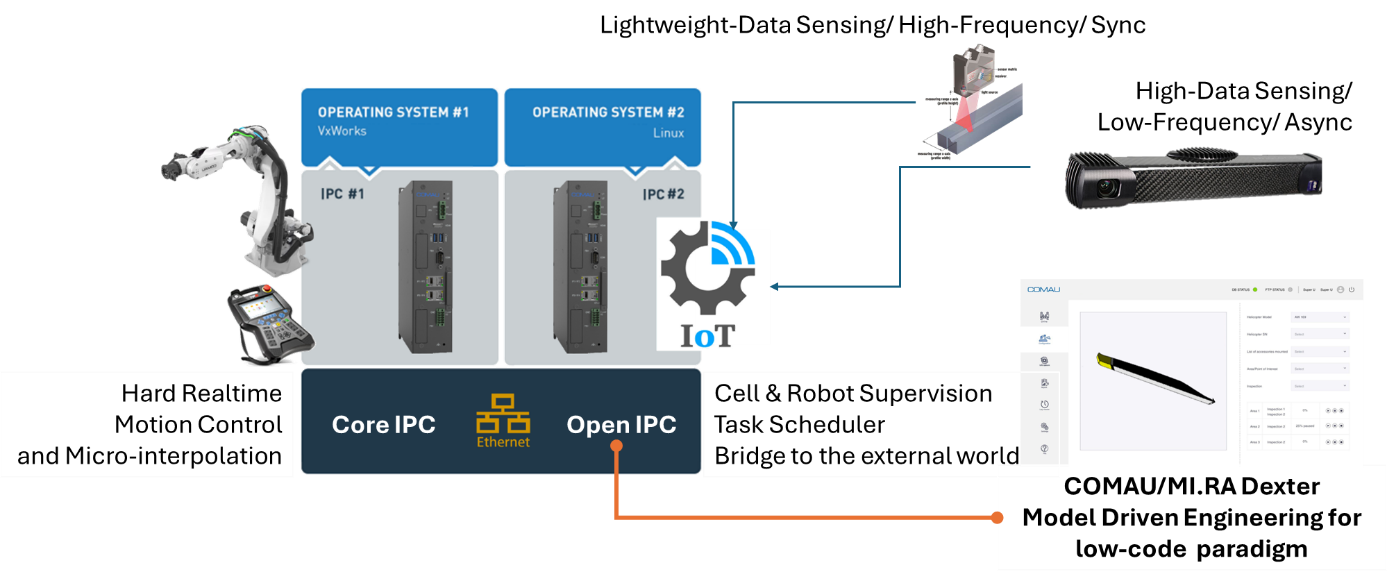
\includegraphics[width=0.9\linewidth]{figures/ipc_architecture.png}
\caption{Baseline architecture of the new generation of robot controllers (from the Project Description): the Open IPC provides programming tools, motion planner and the bridge to cell and sensing; the Core IPC oversees control loops, micro-interpolation and safety rules.}\label{fig:ipc}
\end{figure}

\subsection{Reference application}
Arc welding of very large metal structures by an industrial arm mounted on an AGV (optionally on an interpolated linear axis). The AGV is placed at a station and the arm welds a portion of the structure; base motion interpolated with the arm during welding is a secondary, theoretically relevant option. The task is \emph{under-constrained}: the seam point must be reached exactly, the torch axis may lie within a cone of about $10^\circ$ around the nominal direction (possibly anisotropic between work and travel angle), the rotation about the torch axis is almost always free, and the travel speed must stay constant within $\pm10\%$ along the whole seam. Because of the size of the structure the arm may have to change configuration: stop, retract, reconfigure, approach and restart about 1\,cm before the detach point. Seam segmentation and a raw positioning of the manipulator that reduces reconfiguration risk are standard industrial practice and are made explicit in the updated pipeline.

\subsection{Requirements}\label{sec:req}
\begin{enumerate}[label=R\arabic*.]
\item \textbf{Exact task, free redundancy.} Task constraints (position, axis) are hard; tolerances (cone, roll, external axes, base) are exploited as optimisation freedom~\cite{demaeyer2017descartes,chen2025cooptimization}.
\item \textbf{Speed band.} Travel speed within a fixed band ($\pm10\%$) under joint velocity, acceleration and jerk limits~\cite{lange2016pathaccurate}.
\item \textbf{Planned reconfigurations.} Fewest stop--reconfigure--restart cycles, with planned transfer motions and restart overlap~\cite{yin2024dpbreakpoints,wang2025anytimetracking}.
\item \textbf{Optimal task localisation.} Station / base / rail placement chosen so that whole task segments are feasible~\cite{weingartshofer2021tcpbase,wachter2024tcpbase}.
\item \textbf{Registration.} Mobile platforms on large workpieces show centimetre-level errors without local registration~\cite{zhao2021mobilemachining}; plans are executed on the locally registered task (seam scan~\cite{wang2026torchposture}, Activity~3).
\item \textbf{Human-shared space.} ISO/TS 15066-aware costs and certified speed adaptation~\cite{faroni2022safetyaware,gursoy2026cosmik}.
\item \textbf{Robot-agnostic.} Any serial arm (non-cuspidal or cuspidal~\cite{elias2025cuspidal}), joints with range beyond $\pm\pi$, external linear/rotary axes, mobile bases.
\item \textbf{Industrial integration.} Deterministic, repeatable outputs; dockerised actions in MI.RA/Dexter; hard real-time Core IPC.
\end{enumerate}

\section{Review methodology and evaluation criteria}\label{sec:method}

\subsection{Sources and process}
The review was organised as a version-controlled knowledge base (``LLM wiki''): every source is stored with its full text, a structured summary (method, evidence with table/figure references, relevance, critical assessment) and links to cross-cutting concept pages; bibliographic data are verified on Crossref. Searches covered arXiv (MPPI and sampling-based MPC for manipulators and mobile robots, safety and constraints, multimodality, path-wise redundancy resolution, base placement), IEEE Xplore and Elsevier (welding, redundancy, look-ahead, path following, base placement, multi-robot), SAGE, and the ROS-Industrial documentation of Descartes. Internal project documents (Project Description, D4.1 outline) provided the requirements. At the time of writing the knowledge base contains 119 sources.

\subsection{Inclusion criteria}
In scope: MPPI and path-integral control; sampling-based MPC compared with MPPI; path-wise redundancy resolution and tolerance-aware Cartesian planning; base and task placement; sampling-based planning for manipulators; applications to industrial and collaborative arms, mobile manipulators, AMR/AGV and human-shared spaces; safety and constraint handling; CPU/GPU/embedded implementations. Background (classical MPC, DDP, trajectory optimisation, DWA/TEB) is summarised briefly.

\subsection{Comparison criteria}
Success rate; initial-solution time and convergence; path cost; replanning latency; memory and CPU load; scalability with degrees of freedom; smoothness (jerk); constraint satisfaction (joint limits, speed band, task tolerances); number of reconfigurations and stations; safety-induced idle time; reproducibility, open-source maturity, licence and industrial support. Dynamic-scene and multi-agent categories are evaluated separately.

\section{Updated academic state of the art}
\label{sec:sota}

\subsection{Sampling-based optimal planning: state of the art}\label{sec:sbp}

\begin{planbox}
To be completed by the T4.2 team: informed sets, admissible informed and local sampling, adaptive exploration/exploitation, anytime and multi-query planning with path reuse (Project Description, \S A.4.2). The subsections below summarise the elements of the updated review that affect the revised architecture.
\end{planbox}

\subsubsection{Speed of sampling-based planners}
Vectorising forward kinematics and collision checking with CPU SIMD instructions accelerates any sampling-based planner by more than two orders of magnitude, with median planning times of tens of microseconds for a 7-DoF arm on a single core and support for low-power ARM boards~\cite{thomason2024vamp}. GPU-parallel motion generation (parallel IK, geometric planning, particle-based seeding and L-BFGS) plans collision-free arm motions in tens of milliseconds~\cite{sundaralingam2023curobo}. For Plan4ARI this makes sampling-based planning usable inside the online loop, e.g.\ to plan transfer motions for reconfiguration at every cycle, and to evaluate station candidates exhaustively.

\subsubsection{Tolerance-aware Cartesian path planning}
Industrial processes (welding, spraying, machining) prescribe a Cartesian path with tolerances. The reference open-source approach, Descartes, samples each path point within its tolerances, computes all IK solutions and searches a layered graph; its evaluation on arc welding documents memory growth, the absence of any speed model and torch ``jumps'' within the tolerance range~\cite{demaeyer2017descartes}. Extensions handle external axes~\cite{sun2020externalaxis}, anytime refinement around a guide path minimising reconfigurations~\cite{wang2025anytimetracking}, dynamic programming with an explicit breakpoint cost~\cite{yin2024dpbreakpoints}, global co-optimisation of tool orientation, redundancy and timing~\cite{chen2025cooptimization} and warm-started optimisation with tolerance windows~\cite{weingartshofer2023pathframework}. These are the deterministic baselines of the revised plan.

\subsubsection{Task localisation and base placement}
Base placement has evolved from reachability maps~\cite{makhal2018reuleaux} to set-cover formulations minimising the number of stations~\cite{nguyen2023taskclustering}, placement for sets of continuous paths~\cite{weingartshofer2021tcpbase}, joint base--path optimisation~\cite{zhao2025bstar} and placement scored by true cycle time~\cite{wachter2024tcpbase}. None checks constant-speed feasibility or orientation cones at station level, which motivates stage P2 of the pipeline (Section~\ref{sec:pipeline}).

\subsubsection{Sampling-based planners guiding local optimisers}
Planner-provided nominal trajectories improve the sample efficiency of MPPI~\cite{tao2023rrtmppi}; MPPI can also mix samples from arbitrary ancillary controllers, including global planners~\cite{trevisan2024biasedmppi}. This is the mechanism by which the T4.2 planner and the MPPI look-ahead are coupled.

\subsection{Dynamic replanning and human-aware safety}\label{sec:safety}

\subsubsection{Safety-aware objectives}
ISO/TS 15066 speed-and-separation monitoring and power-and-force limiting reduce the robot speed near humans. Converting these limits into a time-dilation cost lets a planner minimise the \emph{expected execution time including safety slowdowns}; on a real collaborative cell this reduced the robot time by 19\%~\cite{faroni2022safetyaware}. The same principle with biomechanical limits is applied in graph search~\cite{laha2023sstar} and in convex, jerk-limited re-timing along a fixed path~\cite{palleschi2021fastsafe}. These per-configuration costs are non-smooth and naturally evaluated on MPPI rollouts.

\subsubsection{Reactive, risk-aware and constraint-aware sampling}
Recent MPPI variants enforce human separation by terminating violating rollouts at a constant 22\,ms per cycle on a torque-controlled arm~\cite{gursoy2026cosmik}, evaluate collision probabilities against non-Gaussian human predictions for crowds~\cite{trevisan2025drampi}, keep a contingency plan available at all times~\cite{jung2024contingency}, and satisfy kinematic constraints exactly by projection~\cite{lee2026prmppi}. Torque-level MPPI provides compliant behaviour for physical interaction~\cite{im2026torquemppi}.

\subsubsection{Implications}
Safety-aware costs are evaluated in the Open IPC (MPPI rollouts, planner edges) to \emph{anticipate} safety interventions, while the certified speed adaptation and safety rules remain in the Core IPC. Path switching and fallback strategies are provided by the multi-goal look-ahead and by the deterministic plan of each segment (Section~\ref{sec:selected}). Interfaces: human tracking from Activity~3, task alternatives and allocation from Activity~2.

\subsection{Model predictive control and MPPI for trajectory generation}\label{sec:mpc}

This section reports the state of the art on Model Predictive Path Integral (MPPI) control and its relation to MPC, then the industrial look-ahead and path-following methods relevant for the Core-IPC micro-interpolator.

% --- MPPI state of the art, shared with the standalone SOTA note (../SOTA/latex/sota_body.tex)
\begingroup
\let\section\subsubsection
\let\subsection\paragraph
\renewcommand{\paragraph}[1]{\par\runin{#1}}
\input{sota_body}
\endgroup

\subsubsection{Industrial look-ahead, path following and micro-interpolation}
Industrial controllers adapt the speed along a buffered path under kinematic limits. A path-accurate online trajectory generator modifies only the time law of a sampled joint path under velocity, acceleration and jerk limits at 250\,Hz on an industrial controller~\cite{lange2016pathaccurate}; CNC-style Cartesian look-ahead blends corners and scans speed limits bidirectionally~\cite{ma2025lookahead}. Model predictive path-following control treats the path parameter as a virtual state and was solved in at most 0.48\,ms at 1\,kHz on an industrial arm~\cite{faulwasser2017pathfollowing}. Predictive inverse kinematics with task scaling and predictive joint trajectory scaling~\cite{faroni2019pik,faroni2020scaling} and null-space NMPC~\cite{sun2024nullspacempc} are the deterministic counterparts of the MPPI look-ahead. Together they define the path--velocity layer of the Core IPC (Section~\ref{sec:arch}): the joint path is fixed upstream, the time law is optimised within the process speed band under hard limits, and band violations are reported upstream instead of producing unplanned stops.

\subsection{Software frameworks and industrial toolchain}\label{sec:software}

\begin{table}[h]
\centering\small
\caption{Framework matrix (candidates for the Plan4ARI toolchain).}\label{tab:frameworks}
\begin{plangrid}{|L{3.0cm}|L{3.3cm}|Y|L{2.6cm}|}
\planheadrow \thead{Tool} & \thead{Language / hardware} & \thead{Scope} & \thead{Role in Plan4ARI}\\ \hline
OMPL / MoveIt\,2 & C++, CPU & sampling-based planners, ROS\,2 integration & KPI baseline (proposal) \\ \hline
VAMP~\cite{thomason2024vamp} & C++/Python, CPU SIMD & vectorised sampling-based planning & transfers, station checks, rollout primitives \\ \hline
Descartes~\cite{demaeyer2017descartes} & C++, ROS & tolerance-aware Cartesian path planning & deterministic baseline \\ \hline
cuRobo~\cite{sundaralingam2023curobo} & CUDA & GPU motion generation & GPU track baseline \\ \hline
MPPI-Generic~\cite{vlahov2024mppigeneric} & CUDA C++ & MPPI, Tube-MPPI, RMPPI & GPU MPPI reference \\ \hline
STORM~\cite{bhardwaj2021storm} & PyTorch, GPU & joint-space MPPI for arms & MPPI reference \\ \hline
Nav2 MPPI controller~\cite{macenski2023nav2survey} & C++, CPU & AMR local control & AMR baseline \\ \hline
acados~\cite{verschueren2022acados} & C, code generation & embedded NMPC & Core-IPC MPC candidate \\ \hline
Isaac Gym / MuJoCo-MJX~\cite{makoviychuk2021isaacgym,dierking2026parallelsbmpc} & GPU physics & simulator-in-the-loop sampling MPC & simulation benchmarks \\ \hline
MI.RA/Dexter (COMAU) & dockerised actions & low-code platform, digital twin & integration target (T4.4) \\ \hline
\end{plangrid}
\end{table}

Logging, benchmarking, continuous integration and traceability are handled in T4.6 and in the benchmark repository (Section~\ref{sec:bench}).

\section{Gap analysis against the original Plan4ARI plan}\label{sec:gap}

\subsection{What changes with respect to the proposal}
\begin{table}[h]
\centering\small
\caption{Original plan (Project Description, \S A.4 and \S E.3) versus updated plan.}\label{tab:delta}
\begin{plangrid}{|L{3.0cm}|Y|Y|}
\planheadrow \thead{} & \thead{Original plan} & \thead{Updated plan} \\ \hline
Global / online planning (T4.2) & Informed sampling-based planner, mixed global/local sampling, multi-path reuse & \textbf{Retained}; also used for transfer motions (retract, reconfigure, approach) and station-level feasibility; vectorised CPU primitives~\cite{thomason2024vamp} \\ \hline
Local reactive layer & MPC ``alongside'' the sampling-based planner & \textbf{New: MPPI look-ahead} over the task null space with multiple goals, guided by the sampling-based planner~\cite{trevisan2024biasedmppi,tao2023rrtmppi} \\ \hline
Micro-interpolation (T4.3) & MPC in the Core IPC, speed override, visual servoing & \textbf{Retained}; specified as path--velocity layer with hard limits and speed band~\cite{faulwasser2017pathfollowing,lange2016pathaccurate,faroni2020scaling} \\ \hline
Task localisation & Implicit (industrial practice) & \textbf{Explicit pipeline stage}: optimal placement of robot / AGV / external axis~\cite{weingartshofer2021tcpbase,nguyen2023taskclustering} \\ \hline
Safety-aware cost & ISO/TS 15066 cost in the replanner~\cite{faroni2022safetyaware} & \textbf{Retained}; evaluated per rollout and per planner edge \\ \hline
Robot dependence & COMAU platform & \textbf{Robot-agnostic} kinematic abstraction \\ \hline
Benchmarking (T4.7) & $\geq$50 scenarios, OMPL baseline, GPU planners not compared & Same KPIs; application catalogue; welding on hardware, others in simulation; GPU methods in a separate track \\ \hline
\end{plangrid}
\end{table}


\section{Updated scientific and technical architecture}\label{sec:arch}

\subsection{Updated approach: sampling-based planning and MPPI}
Industrial controllers rely on look-ahead: a buffer of future path samples is analysed to adapt speed under kinematic limits~\cite{lange2016pathaccurate}. For under-constrained tasks this look-ahead is limited to a single, pre-computed joint solution. MPPI acts as a \emph{stochastic look-ahead} that explores the redundancy ahead of the robot: it samples many short futures of the null-space variables (torch roll, cone tilt, external axis), evaluates them with arbitrary, non-smooth costs (collisions with the structure, joint-limit and singularity margins, ISO/TS 15066 slowdown, speed feasibility) and returns an improved plan every cycle~\cite{williams2018tro}. Null-space sampling with exact task satisfaction~\cite{wang2024constrainedpi,lee2026prmppi}, its deterministic counterpart~\cite{sun2024nullspacempc} and planner-guided MPPI~\cite{tao2023rrtmppi,trevisan2024biasedmppi} support this choice. Sampling-based planning remains essential where MPPI is weak: long transfer motions in clutter, station-level feasibility and multi-path reuse. \emph{The sampling-based planner proposes, MPPI refines and reacts, the Core-IPC MPC certifies.}

\subsubsection{Multi-goal MPPI look-ahead}
The goal of the look-ahead is a Cartesian task segment (e.g.\ ${\sim}10$\,cm of seam) with a \emph{set of start configurations}, one per inverse-kinematics solution class (up to 8 for a non-cuspidal 6R arm, up to 16 for cuspidal arms, multiplied by joint turns where ranges exceed $\pm\pi$~\cite{elias2025cuspidal}). For each class MPPI optimises the null-space variables along the segment with exact IK on that class. Classes are \emph{selected, never blended}~\cite{liu2026clusteringmppi,wang2026mppiem}. Continuing on the current class has no transfer cost; switching class costs a transfer (planned by the sampling-based planner first to the nominal start for a cost estimate, then to the optimised start, with a consistency check) plus the restart overlap. The time-dilation factor $\lambda=\max_j |\dot q_j^{\mathrm{req}}|/\dot q_j^{\max}$ along each rollout measures speed feasibility ($\lambda\le 1/0.9$ for a $\pm10\%$ band), so that a reconfiguration emerges from cost comparison when the current class cannot keep the speed or approaches joint limits.

\subsection{End-to-end pipeline}\label{sec:pipeline}
\begin{figure}[h]
\centering
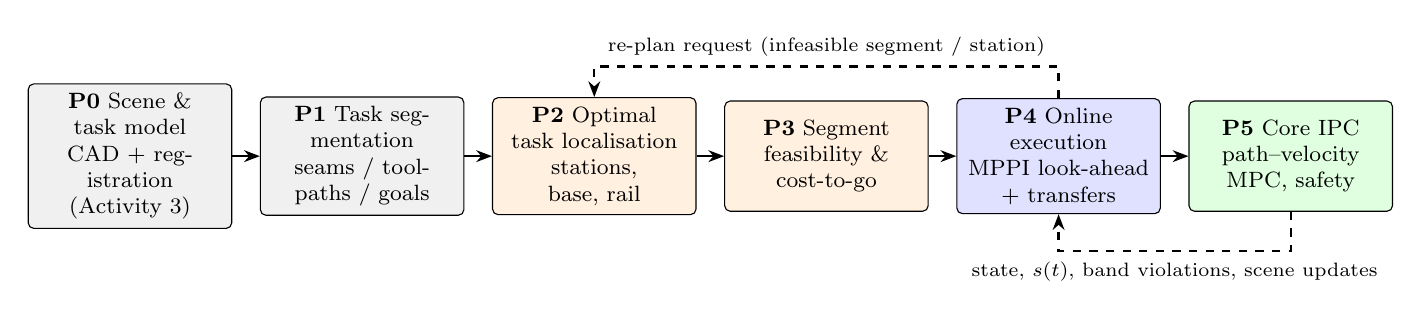
\begin{tikzpicture}[font=\footnotesize, node distance=3.5mm,
  st/.style={draw,rounded corners=2pt,align=center,text width=2.35cm,minimum height=14mm,fill=#1!12},
  arr/.style={-{Stealth[length=2mm]},thick}]
\node[st=gray] (p0) {\textbf{P0} Scene \& task model\\CAD + registration\\(Activity 3)};
\node[st=gray, right=of p0] (p1) {\textbf{P1} Task segmentation\\seams / toolpaths / goals};
\node[st=orange, right=of p1] (p2) {\textbf{P2} Optimal task localisation\\stations, base, rail};
\node[st=orange, right=of p2] (p3) {\textbf{P3} Segment feasibility \& cost-to-go};
\node[st=blue, right=of p3] (p4) {\textbf{P4} Online execution\\MPPI look-ahead + transfers};
\node[st=green, right=of p4] (p5) {\textbf{P5} Core IPC\\path--velocity MPC, safety};
\foreach \a/\b in {p0/p1,p1/p2,p2/p3,p3/p4,p4/p5} \draw[arr] (\a) -- (\b);
\draw[arr,dashed] (p5.south) -- ++(0,-5mm) -| node[pos=0.25,below]{\scriptsize state, $s(t)$, band violations, scene updates} (p4.south);
\draw[arr,dashed] (p4.north) -- ++(0,4mm) -| node[pos=0.25,above]{\scriptsize re-plan request (infeasible segment / station)} (p2.north);
\end{tikzpicture}
\caption{End-to-end pipeline. Orange: planning before execution (Open IPC, seconds to minutes). Blue: online planning (Open IPC, 10--100\,Hz). Green: hard real time (Core IPC, 1\,kHz).}\label{fig:pipeline}
\end{figure}

\begin{description}[leftmargin=0pt]
\item[P0 -- Scene and task model.] CAD of workpiece and cell registered with the sensing modules of Activity~3; local registration at each station (R5).
\item[P1 -- Task segmentation.] Segments with homogeneous constraints (welding: seams split at corners, interruptions and process changes; corners at constant speed are where joint-speed limits break~\cite{gautier2024weldingbase}).
\item[P2 -- Optimal task localisation.] Minimum set of stations (AGV poses, rail intervals or fixed base) such that each segment is \emph{path-wise feasible} from at least one station: set-cover over segments~\cite{nguyen2023taskclustering} with a continuous-branch test~\cite{weingartshofer2021tcpbase}, the speed check $\lambda$, margins for positioning error and orientation tolerances; candidates from inverse reachability maps~\cite{makhal2018reuleaux} and joint base--path optimisation~\cite{zhao2025bstar}.
\item[P3 -- Segment feasibility and cost-to-go.] Per station and segment: feasible IK classes, nominal null-space seeds, reconfiguration points and a cost-to-go table from a deterministic layered-graph / dynamic-programming planner~\cite{yin2024dpbreakpoints,demaeyer2017descartes}; sequence of segments and transfers (with Activity~2 for multi-robot allocation~\cite{tang2023dualrobotweld}).
\item[P4 -- Online execution.] Multi-goal MPPI look-ahead on the registered segment with the P3 cost-to-go as terminal cost; transfers by the T4.2 planner; reaction to scene changes and humans.
\item[P5 -- Core IPC.] Path--velocity layer: the joint path $q(s)$ from P4 is time-parametrised within the speed band under hard limits; speed override and ISO/TS 15066 rules; synchronous sensor input (seam tracking, visual servoing). A band violation is reported upstream as a detach request.
\end{description}

\subsection{Open IPC / Core IPC allocation}\label{sec:ipc}
\begin{figure}[h]
\centering
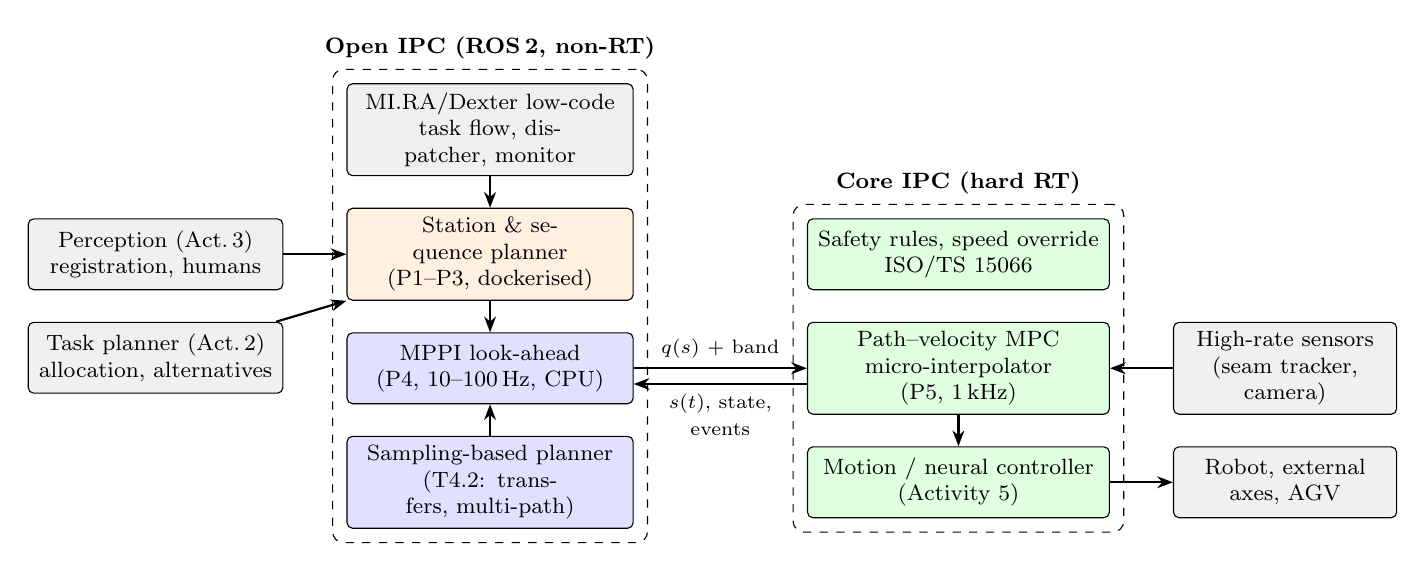
\begin{tikzpicture}[font=\footnotesize,
  blk/.style={draw,rounded corners=2pt,align=center,fill=#1!12,minimum height=9mm},
  arr/.style={-{Stealth[length=2mm]},thick},
  zone/.style={draw,dashed,rounded corners=4pt,inner sep=5pt}]
\node[blk=gray,text width=3.4cm] (dex) at (0,0) {MI.RA/Dexter low-code\\task flow, dispatcher, monitor};
\node[blk=orange,text width=3.4cm,below=4mm of dex] (sta) {Station \& sequence planner\\(P1--P3, dockerised)};
\node[blk=blue,text width=3.4cm,below=4mm of sta] (mppi) {MPPI look-ahead\\(P4, 10--100\,Hz, CPU)};
\node[blk=blue,text width=3.4cm,below=4mm of mppi] (sbp) {Sampling-based planner\\(T4.2: transfers, multi-path)};
\node[blk=gray,text width=3.0cm,left=8mm of sta] (perc) {Perception (Act.\,3)\\registration, humans};
\node[blk=gray,text width=3.0cm,below=4mm of perc] (task) {Task planner (Act.\,2)\\allocation, alternatives};
\node[zone,fit=(dex)(sta)(mppi)(sbp),label={[font=\footnotesize\bfseries]above:Open IPC (ROS\,2, non-RT)}] (open) {};
\node[blk=green,text width=3.6cm,right=22mm of mppi] (mpc) {Path--velocity MPC\\micro-interpolator (P5, 1\,kHz)};
\node[blk=green,text width=3.6cm,above=4mm of mpc] (saf) {Safety rules, speed override\\ISO/TS 15066};
\node[blk=green,text width=3.6cm,below=4mm of mpc] (ctl) {Motion / neural controller\\(Activity 5)};
\node[zone,fit=(saf)(mpc)(ctl),label={[font=\footnotesize\bfseries]above:Core IPC (hard RT)}] (core) {};
\node[blk=gray,text width=2.6cm,right=8mm of ctl] (rob) {Robot, external axes, AGV};
\node[blk=gray,text width=2.6cm,above=4mm of rob] (sens) {High-rate sensors\\(seam tracker, camera)};
\draw[arr] (mppi.east) -- node[above]{\scriptsize $q(s)$ + band}(mpc.west);
\draw[arr] ([yshift=-2mm]mpc.west) -- node[below,align=center]{\scriptsize $s(t)$, state,\\ \scriptsize events} ([yshift=-2mm]mppi.east);
\draw[arr] (mpc) -- (ctl); \draw[arr] (ctl) -- (rob); \draw[arr] (sens) -- (mpc.east);
\draw[arr] (perc) -- (sta); \draw[arr] (task) -- (sta.south west);
\draw[arr] (sta) -- (mppi); \draw[arr] (sbp) -- (mppi); \draw[arr] (dex) -- (sta);
\end{tikzpicture}
\caption{Allocation of the pipeline to the two computing units.}\label{fig:ipcalloc}
\end{figure}

\begin{table}[h]
\centering\small
\caption{Function allocation, rates and interfaces (timing budgets are targets to be confirmed in T4.6/T4.7).}\label{tab:alloc}
\begin{plangrid}{|L{3.6cm}|L{1.5cm}|L{2.5cm}|Y|}
\planheadrow \thead{Function} & \thead{Unit} & \thead{Rate / latency} & \thead{Interface} \\ \hline
Segmentation, task localisation, cost-to-go (P1--P3) & Open IPC & seconds--minutes, before execution & Dockerised MI.RA/Dexter actions; input CAD + registration; output stations, sequence, IK classes, cost-to-go \\ \hline
Sampling-based planner (T4.2) & Open IPC & $\mu$s--ms per query (CPU SIMD~\cite{thomason2024vamp}) & Service: start/goal configuration $\to$ time-parametrised path + cost \\ \hline
MPPI look-ahead (P4) & Open IPC & 10--100\,Hz & Streams $q(s)$ over a horizon of the segment, admissible speed band, mode/detach events \\ \hline
Path--velocity MPC (P5) & Core IPC & 1\,kHz, deterministic & Async channel from Open IPC; sync channel from sensors; hard channel to drives~\cite{faulwasser2017pathfollowing} \\ \hline
Safety / speed override & Core IPC & 1\,kHz & ISO/TS 15066 limits, human data from Activity 3~\cite{faroni2022safetyaware} \\ \hline
\end{plangrid}
\end{table}

\runin{Design rules.} (i) Everything stochastic runs in the Open IPC; the Core IPC receives smooth references and enforces hard limits deterministically. (ii) The MPPI layer runs on CPU by default (vectorised kinematics and collision checking~\cite{thomason2024vamp}) to stay comparable with the OMPL-based KPI; GPU execution is a separately reported variant. (iii) Every online plan has a deterministic fallback: the P3 plan of the current segment. (iv) Fixed-seed, low-discrepancy sampling and logging make execution repeatable for process qualification.

\subsection{Robot-agnostic design}\label{sec:agnostic}
The framework is parametrised by a \emph{kinematic description} (URDF, joint ranges, external axes, base model) and a \emph{task description} (constraint type per Cartesian degree of freedom: exact, band, cone, free). From these it derives automatically: the IK solver class --- analytic where available (6R families, including cuspidal arms~\cite{elias2025cuspidal}), numerical functional-redundancy IK otherwise~\cite{razjigaev2025functional} --- and the set of \emph{solution classes} used as goals (branches $\times$ joint turns); the null-space coordinates sampled by MPPI (tool roll, cone tilts, external axes, redundant joints, base); collision geometry (sphere approximations for vectorised checking) and kinematic limits. Supported configurations: fixed arms, arms on linear or rotary axes, arms on AGVs (base fixed per station or interpolated), dual-arm and multi-robot cells~\cite{ye2026nullspacemultirobot}.

\subsection{First mockup scope and demonstration evidence}\label{sec:mockup}
The M12 mockup is the initial implementation of the motion planning workflow, rather than the completed industrial integration planned for Tasks~4.4 and~4.5. The proposed demonstration uses the reference welding scenario in a simulated cell: registered geometry and task constraints are supplied as inputs; the station and segment planners produce feasible configurations and a nominal path; sampling-based planning generates transfer motions; MPPI explores task redundancy; and a deterministic path--velocity component checks the resulting reference against the configured limits. An unavailable component must be identified explicitly as a stub or an offline computation in the demonstration record.

The review package should include the software revision and dependency versions, robot and cell models, task parameters, a reproducible launch procedure, fixed random seeds, planning and execution logs, a demonstration recording, and a list of implemented and pending interfaces. The initial checks concern collision-free feasibility, Cartesian task tolerances, the nominal process speed band, joint limits and stationary behaviour when planning fails. The initial static, kinematic scope and the planned MPPI integration are specified in Sections~\ref{sec:simenv} and~\ref{sec:simtimeline}. Measured latency and violations must be reported against the benchmark protocol of Section~\ref{sec:bench}. The M12 demonstration is distinct from subsequent hardware validation, the M24 prototypes and the M36 COMAU IPC integration.
\section{Method selection and decision rationale}\label{sec:selected}

\begin{table}[h]
\centering\small
\caption{Method-selection record.}\label{tab:methods}
\begin{plangrid}{|L{2.6cm}|Y|L{3.7cm}|L{2.5cm}|}
\planheadrow \thead{Function} & \thead{Selected approach} & \thead{Baselines} & \thead{Fallback} \\ \hline
Task localisation (P2) & Set-cover over segments with path-wise feasibility test & Point-based placement~\cite{makhal2018reuleaux,nguyen2023taskclustering}; optimisation-based~\cite{zhao2025bstar,weingartshofer2021tcpbase} & Operator-defined stations \\ \hline
Segment feasibility, cost-to-go (P3) & Layered graph / DP over IK classes and discretised null space, breakpoint cost & Descartes~\cite{demaeyer2017descartes}; anytime tracking~\cite{wang2025anytimetracking}; co-optimisation~\cite{chen2025cooptimization} & Single-class DP \\ \hline
Transfer and global planning (T4.2) & Informed sampling with mixed global/local sampling and multi-path reuse, vectorised primitives & OMPL planners; VAMP~\cite{thomason2024vamp} & Pre-taught via-points \\ \hline
Online look-ahead (P4) & Multi-goal null-space MPPI, exact IK per class, select-never-blend, planner-guided & Null-space NMPC~\cite{sun2024nullspacempc}; predictive IK~\cite{faroni2019pik}; P3 plan replay & P3 plan + speed scaling \\ \hline
Micro-interpolation (P5, T4.3) & Path--velocity MPC with speed band and hard limits & Path-accurate OTG~\cite{lange2016pathaccurate}; trajectory scaling~\cite{faroni2020scaling,palleschi2021fastsafe} & Speed override only \\ \hline
Human-aware cost & ISO/TS 15066 time-dilation cost~\cite{faroni2022safetyaware}; risk-aware rollouts~\cite{trevisan2025drampi} & Plain SSM speed scaling & Safety stop \\ \hline
\end{plangrid}
\end{table}

\runin{Verification obligations.} Exact task tracking and hard limits are guaranteed by construction (exact IK per class, Core-IPC MPC); MPPI provides performance, not certification. Optimality and completeness claims are attached to the deterministic layers (P3, T4.2 planner). Fallbacks cover infeasible optimisation (P3 plan), missed deadlines (speed scaling in the Core IPC) and degraded sensing (stop at the next planned detach point).

\section{Benchmarking and validation plan}\label{sec:bench}

\begin{planbox}
The methods are evaluated on a broad catalogue of industrial applications sharing the structure ``under-constrained task + speed requirements + possible base/axis redundancy + dynamic, human-shared scene''. \textbf{Arc welding of large structures is the only application planned for validation on real hardware} (reference demonstrator); \textbf{all other applications are planned for benchmarking in simulation}, on digital twins (COMAU virtualisation tools and open simulators), across several robot kinematic classes (R7).
\end{planbox}

\subsection{Application catalogue}
{\small\renewcommand{\arraystretch}{1.25}
\begin{longtable}{|L{2.8cm}|L{4.4cm}|L{2.9cm}|L{2.6cm}|L{1.2cm}|}
\caption{Application catalogue for Task 4.7 (R = real hardware, S = simulation).}\label{tab:apps}\\ \hline
\planheadrow \thead{Application} & \thead{Task structure / redundancy} & \thead{Platform} & \thead{Key metrics} & \thead{Eval.} \\ \hline\endfirsthead
\hline\planheadrow \thead{Application} & \thead{Task structure / redundancy} & \thead{Platform} & \thead{Key metrics} & \thead{Eval.} \\ \hline\endhead
Arc welding of large structures & 5-DoF seam, cone, free roll, constant speed $\pm10\%$, reconfigurations & 6-axis arm on AGV, optional rail & restarts, speed band, angles & \textbf{R} + S \\ \hline
Multi-robot welding & synchronous / ordered seams, shared workspace~\cite{tang2023dualrobotweld} & 2+ arms, AGVs & cycle time, waiting, collisions & S \\ \hline
Spray painting / coating & 5-DoF, free roll about nozzle, stand-off band~\cite{weingartshofer2023pathframework} & arm, rail & coverage, speed band & S \\ \hline
Cold / thermal spray & 5-DoF toolpath, functional redundancy~\cite{razjigaev2025functional} & arm & joint travel, speed & S \\ \hline
Sealing / gluing / dispensing & 5-DoF, constant speed, corners & arm, AGV & speed band, path error & S \\ \hline
Deburring / grinding / sanding & 5-DoF, contact force, large parts~\cite{zhao2021mobilemachining} & mobile manipulator & path error, force, stations & S \\ \hline
Milling / trimming / machining & 5-DoF, stiffness, smooth tool axis~\cite{yang2024toolpathsmoothing,lu2022toolorientation} & arm, positioner, dual arm~\cite{ye2026nullspacemultirobot} & error, jerk, cycle time & S \\ \hline
Polishing & 5-DoF, contact, cone & arm & speed, force & S \\ \hline
Laser cutting / laser welding & 5-DoF, tight speed tolerance & arm, gantry & speed band, error & S \\ \hline
Drilling / riveting (aerospace) & point targets with tool axis, many stations~\cite{nguyen2023taskclustering} & mobile manipulator & stations, cycle time & S \\ \hline
Ultrasound / NDT inspection & surface following with bounded offsets~\cite{yin2024dprealtime} & arm, AGV & coverage, offsets & S \\ \hline
Wire-arc additive manufacturing & 5-DoF layers, free roll~\cite{dharmawan2018functional} & arm, positioner & speed, joint travel & S \\ \hline
Fibre / tape placement & tool normal to surface, redundant cell~\cite{farzanehkaloorazi2018pathplacement} & arm, positioner, axes & singularity margin, time & S \\ \hline
Pick-and-place / palletising & free-space transfers, base placement~\cite{wachter2024tcpbase} & arm, AGV & cycle time, success & S \\ \hline
Machine tending / assembly & transfers in clutter, human access & cobot, AGV & success, latency, idle time & S \\ \hline
Collaborative operations near humans & ISO/TS 15066 SSM/PFL~\cite{faroni2022safetyaware,gursoy2026cosmik} & cobot & idle time ($-30\%$ target), safety stops & S \\ \hline
Intralogistics / AMR fleets & navigation in crowds~\cite{trevisan2025drampi,macenski2023nav2survey} & AMRs, mobile manipulators & success, freezing, time & S \\ \hline
\end{longtable}}

\subsection{Protocol and KPIs}
In line with the proposal: at least 50 application scenarios drawn from Table~\ref{tab:apps}, computation time averaged over more than 100 contexts, OMPL planners as baseline for the sampling-based layer; GPU-based variants reported in a separate track. Additional baselines per layer as in Table~\ref{tab:methods}. Metrics: success rate; planning and replanning latency; number of stations, restarts and reconfigurations; deviation from the speed band; task-tolerance usage (work/travel angles); joint-limit and singularity margins; path accuracy; cycle time; safety-induced idle time and safety stops; smoothness (jerk); CPU/memory load; repeatability across runs. The welding benchmark extends an existing welding motion-planning benchmark framework (weld segments plus transitions)~\cite{demaeyer2021weldbenchmark}. Ablations: with/without MPPI look-ahead, with/without P2 optimisation, horizon length (5/10/20\,cm), number of goals, CPU vs GPU.

\subsection{Benchmark repository}
The benchmark repository has been established within T4.6/T4.7 at \href{https://github.com/CNR-STIIMA-IRAS/plan4ari_a4_benchmarking}{the Plan4ARI A4 benchmarking repository}. It will collect scenarios, redistributable robot and cell assets, task descriptions, baselines and evaluation scripts. The \href{https://github.com/CNR-STIIMA-IRAS/plan4ari_a4_benchmarking/blob/master/docs/architecture.md}{architecture and dependency design document} is the reference for implementation details and technical validation checks; the design summarised here corresponds to repository revision \texttt{dea82b3}. Establishing the repository and design does not constitute evidence of a completed simulator.

\subsection{Simulation environment design}\label{sec:simenv}
The initial A4 benchmark uses static scenes and purely kinematic simulation. ROS\,2 provides the integration layer, a behaviour tree specifies the application sequence, and interchangeable planner adapters separate task logic from planning algorithms. MuJoCo provides the kinematic scene and trajectory replay; OMPL is the transfer-planning baseline, while Tesseract/Descartes provides the proposed Cartesian process-planning baseline, with TrajOpt refinement evaluated subsequently. Time parameterisation and independent validation check the prescribed process speed, Cartesian tolerances, joint limits and collision-free feasibility. The target development platform is Ubuntu~26.04 with ROS\,2 Lyrical, used both in WSL and on native Ubuntu. The initial environment is CPU-only and targets machines with at most 32\,GB RAM; dependency and model compatibility remain subject to prototype validation.

The first application uses the COMAU N-220-2.7 and a synthetic shipbuilding panel with stiffeners and parameterised weld seams. The available USD robot asset must be converted and validated for the planning and simulation representations. The initial robot support is fixed; a modular heavy mobile base and multiple workstations are subsequent extensions. Authorised industrial geometry will be added when supplied by COMAU. A complete plan must be validated before motion starts: if planning fails, times out or returns an invalid plan, the robot remains stationary and the welding process is inactive, without automatic recovery motions.

All planners are evaluated on the same contexts and budgets. Successes, timeouts and failures are reported for all attempts; nominal trajectory quality and execution time are evaluated on successful runs, with results separated by scenario type and difficulty. A local dashboard supports comparison and inspection. GitHub stores code, configurations and redistributable assets; SharePoint stores completed campaign data and reports. Dynamic-scene handling is deferred to the subsequent A3 revision, and dynamics, actuation and control modelling to the A6 revision. Consequently, the initial results describe nominal kinematic performance, not dynamic tracking, contact forces or physical stability.

\section{COMAU contributions to industrial design}\label{sec:comau}
\subsection{Industrial platform and integration requirements}
MI.RA/Dexter and the Open IPC / Core IPC separation are the industrial baseline for Activity~4. COMAU input is required to confirm the robot and external-axis models, available motion interfaces, execution and monitoring semantics, computing budgets, and the constraints on deployment in the industrial controller. The existing platform is distinguished from project-specific design contributions.

\subsection{Contribution traceability and mockup review}
The reporting record should link each confirmed contribution to its source, the resulting design decision and the affected mockup artefact. Candidate contributions concern selection of the welding use case, process tolerances and restart rules, validation of the allocation in Section~\ref{sec:ipc}, review of the demonstration and benchmark protocol, and interface preparation for Tasks~4.4 and~4.5. These categories are proposed for confirmation; they do not certify completed work or assign personnel effort. Review outcomes should record the date, participants, accepted changes and remaining actions.
\section{Updated implementation roadmap}\label{sec:roadmap}

\subsection{Mapping onto Tasks 4.2--4.7}
\begin{itemize}
\item \textbf{T4.2} (M4--M24): informed sampling-based planner with mixed sampling and multi-path reuse (as proposed); in addition, vectorised CPU primitives, transfer motions for reconfiguration, station-level feasibility (P2--P3) and the MPPI look-ahead (P4), including its guidance by the sampling-based planner.
\item \textbf{T4.3} (M4--M24): path--velocity MPC micro-interpolator (P5) with speed band, hard limits, Cartesian/joint interfaces and synchronous sensor input (as proposed); interface to the MPPI layer.
\item \textbf{T4.4} (M25--M30): integration of P1--P4 as dockerised MI.RA/Dexter actions.
\item \textbf{T4.5} (M31--M36): integration of P5 in the COMAU Core IPC.
\item \textbf{T4.6} (M4--M36): continuous integration, including the benchmark repository.
\item \textbf{T4.7} (M1--M6, then continuous): application catalogue, scenarios and protocol (Section~\ref{sec:bench}).
\end{itemize}
Interfaces and dependencies: Activity~2 (task alternatives, multi-robot allocation), Activity~3 (registration, human tracking, seam sensing), Activity~5 (motion/neural control in the Core IPC), Activity~7 (demonstrator).

\subsection{Simulation environment and MPPI implementation timeline}\label{sec:simtimeline}
The following calendar milestones are planning targets for the environment of Section~\ref{sec:simenv}; they do not replace the contractual task periods or certify completed work. The simulation environment is targeted for completion by December~2026, independently of the MPPI algorithm, whose initial integration is expected around March~2027.

\begin{table}[htbp]
\centering\small
\renewcommand{\arraystretch}{1.2}
\begin{tabular}{|L{2.5cm}|L{5.0cm}|L{6.0cm}|}
\hline
\planheadrow \thead{Target period} & \thead{Implementation milestone} & \thead{Expected evidence} \\ \hline
October 2026 & Validate the software stack, robot representation and synthetic welding cell & Robot kinematics, frames and collision geometry checked; reproducible cell loading and baseline planning \\ \hline
November 2026 & Integrate behaviour-tree execution, planner adapters and nominal trajectory validation & Complete static-scene task; stationary behaviour on planning failure; logs and initial KPI evaluation \\ \hline
December 2026 & Finalise the initial simulation and benchmarking environment & Reproducible CPU campaign with baseline planners, local dashboard and archived results; implemented interfaces and remaining limitations documented \\ \hline
January--February 2027 & Develop MPPI and prepare integration into the established benchmark & Algorithm interfaces, task-redundancy exploration and comparison protocol prepared using the same scenarios and constraints \\ \hline
Around March 2027 & Integrate and evaluate the initial MPPI algorithm & Comparative campaign against the established baselines, including nominal constraint satisfaction, planning cost and reconfiguration metrics \\ \hline
\end{tabular}
\caption{Planned implementation milestones for the initial A4 simulation environment and subsequent MPPI integration.}
\end{table}

The December milestone concerns the initial static, kinematic environment and first welding application, not completion of all application families or hardware validation. MPPI remains pending until its implementation and evaluation are recorded; any earlier mockup must identify its absence explicitly. Subsequent extensions address the broader application catalogue, mobile-base configurations and the separate A3/A6 developments.


\section{Risks, ethics and regulatory alignment}\label{sec:risks}

\subsection{Risks}
\begin{table}[h]
\centering\small
\caption{Main technical risks and mitigations.}\label{tab:risks}
\begin{plangrid}{|L{3.6cm}|Y|}
\planheadrow \thead{Risk} & \thead{Mitigation} \\ \hline
Novelty boundary: null-space sampling MPPI alone is not new~\cite{wang2024constrainedpi} & Claim the combination of online null-space look-ahead with solution-class modes, planned transfers and restarts, speed band, task localisation and Open/Core IPC deployment \\ \hline
Compute budget of MPPI on industrial CPUs & Early micro-benchmark in T4.2; CPU SIMD primitives; GPU as optional track \\ \hline
Accuracy of mobile platforms on large parts~\cite{zhao2021mobilemachining} & Local registration and seam tracking (Activity 3) as prerequisite \\ \hline
Process coupling (restart overlap, speed tolerance) & Parameters agreed with welding process experts; parametric in the planner \\ \hline
KPI comparability (GPU planners excluded from the OMPL comparison) & CPU-first design, separate GPU track \\ \hline
Certification of stochastic planners & Hard limits and safety enforced only in the deterministic Core IPC; repeatable sampling and logging \\ \hline
\end{plangrid}
\end{table}

\subsection{Standards and compliance}
ISO 10218 and ISO/TS 15066 for collaborative operation (speed and separation monitoring, power and force limiting); welding quality requirements (process qualification, repeatability of the executed trajectory); EU AI Act requirements on transparency and safety of AI components, as foreseen by the Project Description.

\subsection{Human oversight and evidence traceability}
The mockup should expose infeasibility, fallback activation and process-limit violations to the operator. Human-tracking data and execution logs require controlled access and retention appropriate to their use. Safety and compliance require system-level assessment; planner cost terms and simulation results alone do not establish certification.

\section{Conclusions and proposed updates}\label{sec:conclusions}

\subsection{Retained and modified methods}
\begin{itemize}
\item Retained: informed sampling-based planning with mixed sampling and multi-path reuse (T4.2); MPC micro-interpolation in the Core IPC (T4.3); ISO/TS 15066 safety-aware cost.
\item Added: MPPI look-ahead with multiple goals over the task null space; explicit optimal task localisation (stations, base, rail); deterministic segment planner providing cost-to-go and fallbacks; robot-agnostic kinematic abstraction.
\item Modified: the Core-IPC MPC is specified as a path--velocity layer with process speed band; the sampling-based planner is also used for transfer motions and station-level checks.
\end{itemize}

\subsection{Proposed benchmark and integration plan}
Application catalogue of Section~\ref{sec:bench}, with welding planned for real-hardware validation and all other applications in simulation; KPIs and OMPL baseline as in the proposal, GPU variants in a separate track; benchmark repository within T4.6/T4.7.

\subsection{Open scientific questions and technology watch}
Horizon length versus number of restarts for the look-ahead; mode selection stability (hysteresis) among solution classes; certification argument for the MPPI + Core-IPC chain; scaling to tightly coupled multi-robot tasks; updates of fast sampling-based planners and of MPPI theory (gradient and expectation--maximisation interpretations~\cite{fazlyab2026mppigd,wang2026mppiem}).

\subsection{Consortium approval record}
\begin{planbox}
To be completed after the consortium review (date, participants, decisions).
\end{planbox}

\clearpage
\bibliographystyle{IEEEtran}
\bibliography{references}
\end{document}
